\newcommand{\QoneCost}{35,126.95}
\newcommand{\QoneGrid}{59,482.70}
\newcommand{\QoneCharge}{20,740.67}
\newcommand{\QoneDischarge}{16,799.94}
\newcommand{\QoneLoss}{3,940.73}
\newcommand{\QoneSaving}{12,925.10}
\newcommand{\QoneSaveRate}{26.90}

\section{问题一：微网日前调度模型}
\label{sec:q1}

\subsection{问题分析}

问题一已知全天电价、负载和光伏预测。储能的当前充放电会影响后续可用电量和光伏存储空间，因此需统一安排全天购电与充放电。

本文以10分钟为步长划分144个区间，以线性规划（LP）求取主结果，并用显式充放电互斥的混合整数线性规划（MILP）及网格动态规划（DP）交叉验证。求解与检验流程见图\ref{fig:q1-workflow}。

\begin{figure}[H]
    \centering
    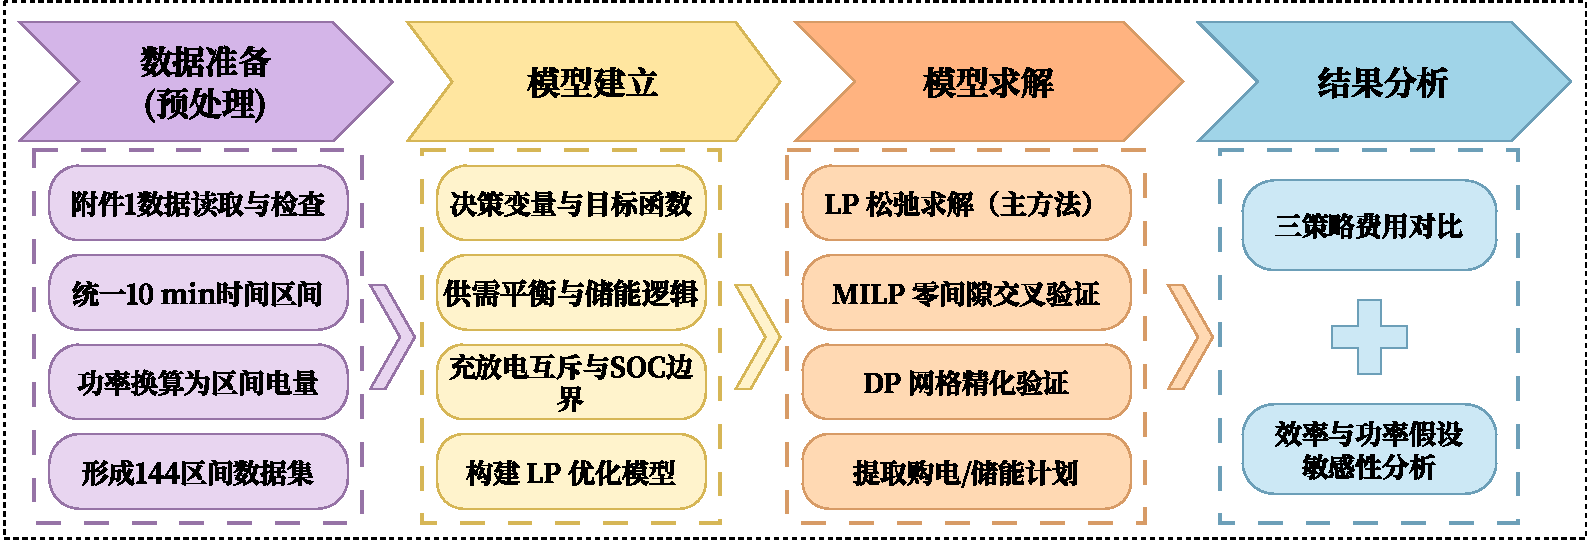
\includegraphics[width=\textwidth]{figures/q1/flowchart1.pdf}
    \caption{问题一流程图}
    \label{fig:q1-workflow}
\end{figure}

\subsection{数据预处理}

\textbf{Step 1：划分时段。}附件1的144条记录各对应此前10分钟。令$t=0,\ldots,143$表示区间$[t\Delta t,(t+1)\Delta t)$，$\Delta t=1/6\,\mathrm h$，共144个供电区间、145个储电量端点，最后一个端点为24:00。

\textbf{Step 2：统一功率与电量。}模型采用区间电量作为决策变量，将附件功率换算为
\begin{equation}
    L_t=P_t^{\mathrm L}\Delta t,\qquad
    V_t=\widehat P_t^{\mathrm{PV}}\Delta t.
    \label{eq:q1-energy}
\end{equation}
其中，$V_t$为光伏预测电量。数据完整，负载与光伏非负、电价为正，直接用于建模。

\subsection{模型建立}

\subsubsection{决策变量与目标函数}

各区间的购电量$q_t$、充电量$c_t$、放电量$d_t$和未利用电量$w_t$均按交流侧$\mathrm{kWh}$计量。$E_t$为区间起点的内部储电量，二元变量$z_t$区分充放电模式，两种模式均允许闲置。

本问售电收入设为0，购电按计划电量与对应时段单价结算，目标为
\begin{equation}
    \min J=\sum_{t=0}^{T-1}p_tq_t,\qquad T=144.
    \label{eq:q1-objective}
\end{equation}
其中$q_t$为区间电量，目标函数单位为元。

\subsubsection{供需平衡与储能运行约束}

\textbf{（1）区间供需平衡。}外网购电、光伏及电池放电共同满足负载与充电需求，富余部分记为未利用电量：
\begin{equation}
    q_t+V_t+d_t=L_t+c_t+w_t,\qquad
    q_t,c_t,d_t,w_t\geq0.
    \label{eq:q1-balance}
\end{equation}
$w_t$为供给超过负载和充电需求的剩余电量，包括未使用的光伏电量与已购电量；购电费按计划计算。

\textbf{（2）储电量递推。}按假设2，充电$c_t$使内部电量增加$\eta_c c_t$，向母线放电$d_t$需消耗内部电量$d_t/\eta_d$，故
\begin{equation}
    E_{t+1}=E_t+\eta_c c_t-\frac{d_t}{\eta_d},
    \qquad \eta_c=\eta_d=0.9.
    \label{eq:q1-soc}
\end{equation}

\textbf{（3）运行电量与首末状态。}设备额定容量为$12000\,\mathrm{kWh}$，可运行范围为其10\%--90\%，要求
\begin{equation}
    \begin{aligned}
        E_{\min}\leq E_t\leq E_{\max},\quad &t=0,\ldots,T,\\
        E_{\min}=1200,\qquad &E_{\max}=10800,\\
        E_0=E_T=E^{\mathrm{init}}&=6000.
    \end{aligned}
    \label{eq:q1-bounds}
\end{equation}
首末电量相等保证电池在日末恢复初始储电量。由于采用区间恒功率近似，内部储电量在每个区间内线性变化，因此，各区间起止时刻的储电量满足上下限时，区间内也满足。

\Needspace{7\baselineskip}
\textbf{（4）充放电功率与模式互斥。}交流侧最大充放电功率$P_{\max}=5000\,\mathrm{kW}$，每个区间的电量上限为$P_{\max}\Delta t=833.3333\,\mathrm{kWh}$。令
\begin{equation}
    \begin{aligned}
        0\leq c_t&\leq P_{\max}\Delta t\,z_t,\\
        0\leq d_t&\leq P_{\max}\Delta t\,(1-z_t),\qquad z_t\in\{0,1\}.
    \end{aligned}
    \label{eq:q1-mode}
\end{equation}
当$z_t=1$时仅允许充电，当$z_t=0$时仅允许放电，从而排除同一区间同时充放电。

\subsection{模型求解}

先去掉二元变量得到LP松弛。若某格同时充放电，可扣除相互抵消的充放电量，保持相同的储电量变化；在电价非负、允许处理富余电量且切换费用为0时，变换后的购电费用小于或等于原费用。因此LP存在同费用的互斥解。保存的LP轨迹经复核已满足互斥，其费用与MILP在数值容差内一致。另采用DP进行网格转移，将储电量网格从50细化至6.25\,kWh时，相对LP下界的费用差距由0.7906\%降至0.0771\%。网格DP提供可行费用上界，LP提供最优费用下界。

\subsection{求解结果}

最终，LP得到全天购电量$\QoneGrid\,\mathrm{kWh}$、最低费用$\QoneCost$元；MILP得到同值并给出零求解间隙。该费用较无储能方案节省$\QoneSaving$元（$\QoneSaveRate\%$），未利用电量为0。低价充电、午间预留光伏存储空间和高峰放电共同降低了费用。

\subsubsection{购电与储能安排}

表\ref{tab:q1-purchase}、表\ref{tab:q1-storage}列出指定时段和全天的购电、储能结果，数值保留两位小数。

\begin{table}[H]
    \centering\small
    \caption{指定时段购电量及全天购电结果（电量单位：kWh）}
    \label{tab:q1-purchase}
    \renewcommand{\arraystretch}{1.2}
    \begin{NiceTabularX}{\textwidth}{
  @{}
  l >{\raggedleft\arraybackslash}p{13mm} X
  l >{\raggedleft\arraybackslash}p{13mm} X
  l >{\raggedleft\arraybackslash}p{13mm}
  @{}
}
\CodeBefore
  \rowcolor{paperpale}{1}
  \rowcolor{paperstripe}{3}
\Body
\toprule
时间段 & 购电量 & & 时间段 & 购电量 & & 时间段 & 购电量 \\
\midrule
10:00--10:10 & 0.00 & & 12:00--12:10 & 480.41 & & 14:00--14:10 & 0.00 \\
16:00--16:10 & 445.43 & & 18:00--18:10 & 531.89 & & 20:00--20:10 & 0.00 \\
\Block[l]{1-*}{
  \makebox[\textwidth][l]{
    全天购电量/kWh\hspace{20mm}59,482.70
    \hfill
    全天购电费/元\hspace{20mm}35,126.95
  }
} & & & & & & & \\
\bottomrule
\end{NiceTabularX}

\end{table}

\begin{table}[H]
    \centering\small
    \caption{指定时段充放电量及首末储电量（单位：kWh）}
    \label{tab:q1-storage}
    \renewcommand{\arraystretch}{1.2}
    \begin{NiceTabularX}{\textwidth}{
  @{}lX[r]X[r]@{\hspace{10mm}}lX[r]X[r]@{}
}
\CodeBefore
  \rowcolor{paperpale}{1}
  \rowcolor{paperstripe}{3,5}
\Body
\toprule
时间段 & 充电量 & 放电量 & 时间段 & 充电量 & 放电量 \\
\midrule
00:00--04:00 & 4,500.00 & 0.00 & 04:00--08:00 & 833.33 & 6,365.84 \\
08:00--12:00 & 4,787.96 & 1,703.00 & 12:00--16:00 & 5,286.04 & 91.10 \\
16:00--20:00 & 0.00 & 5,780.13 & 20:00--24:00 & 5,333.33 & 2,859.87 \\
\Block[l]{1-*}{
  \makebox[\textwidth][l]{
    0:00 储电量\hspace{30mm}6,000.00
    \hfill
    24:00 储电量\hspace{30mm}6,000.00
  }
} & & & & & \\
\bottomrule
\end{NiceTabularX}



\end{table}

全天充电量为$\QoneCharge\,\mathrm{kWh}$，放电量为$\QoneDischarge\,\mathrm{kWh}$。四小时时段内可以先后发生充电和放电，因此两项汇总电量可能均为正；同一10分钟区间内只进行充电或放电。

\subsubsection{调度过程的可视化分析}

\begin{figure}[H]
    \centering
    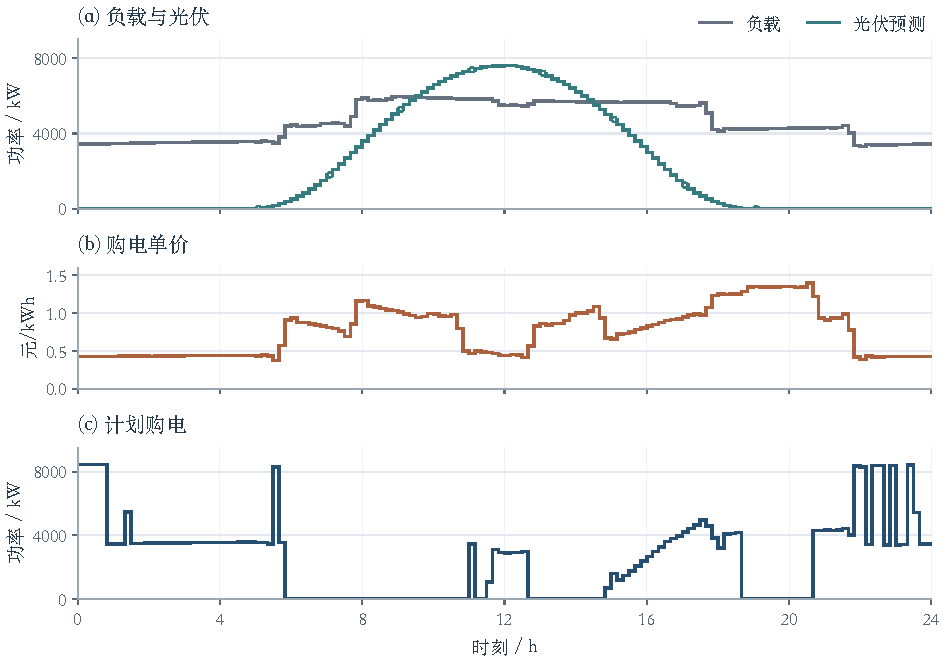
\includegraphics[width=\textwidth]{figures/q1/q1_plan_overview.pdf}
    \caption{负载、光伏、电价与最优购电计划}
    \label{fig:q1-plan-overview}
\end{figure}

\begin{figure}[H]
    \centering
    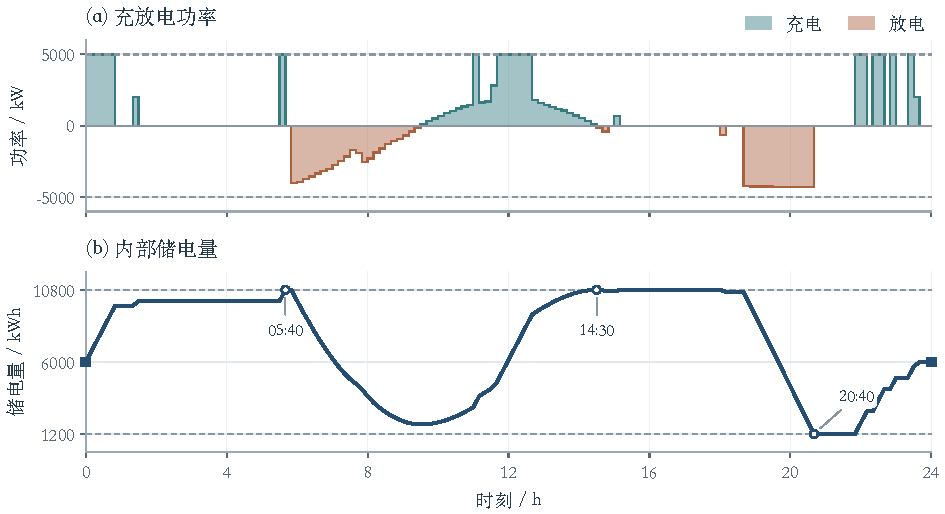
\includegraphics[width=\textwidth]{figures/q1/q1_storage.pdf}
    \caption{储能运行轨迹（充电取正、放电取负）}
    \label{fig:q1-storage}
\end{figure}

图\ref{fig:q1-plan-overview}显示，部分低价时段购电超过负载，用于储能；光伏富余或储能供电充足时，外网购电量为0。图\ref{fig:q1-storage}展示了充放电功率和储电量随时间的变化，标出了储电量上下限、首末电量及达到上下限的时刻。

\Needspace{4\baselineskip}
\textbf{低价充电与早间放电。}05:30--05:40为全天最低价区间，单价为$0.3713$元/kWh，电池以最大允许功率充电，05:40达到$10800\,\mathrm{kWh}$。05:50--09:30外网购电量为0，累计放电$8068.84\,\mathrm{kWh}$，储电量降至$1834.62\,\mathrm{kWh}$，为后续多余的光伏电量留出存储空间。

\textbf{午间购电与光伏储电。}09:30--14:30累计充电$9961.53\,\mathrm{kWh}$，其中同期净光伏富余为$6247.96\,\mathrm{kWh}$、购电为$3713.57\,\mathrm{kWh}$。12:30--12:40虽然处于午间最低价区间并满功率充电，但12:40仍留有$1656.21\,\mathrm{kWh}$内部空间；此后至14:30的$1840.23\,\mathrm{kWh}$净光伏富余，经90\%充电效率转换后恰好填补该空间。模型据此为后续光伏留出空间，同时满足充电功率约束。

\textbf{晚高峰放电与日末恢复。}18:00--20:40累计放电$8640.00\,\mathrm{kWh}$，内部电量由$10800$降至$1200\,\mathrm{kWh}$；21:50后累计充电$5333.33\,\mathrm{kWh}$，24:00恢复至$6000\,\mathrm{kWh}$。受功率上限等因素限制，部分高价时段仍需购电，例如18:00--18:10仍需购电$531.89\,\mathrm{kWh}$。

\subsubsection{不同策略的费用比较}

在相同输入和首末储电量下设置两个对照：无储能方案购买负载超过光伏的部分；固定规则在00:00--06:00尽量充电，16:00后放电补足光伏无法满足的负载，并保留$6000\,\mathrm{kWh}$日末电量。费用见表\ref{tab:q1-comparison}。

\begin{table}[H]
    \centering\small
    \caption{相同首末状态下不同策略的全天费用比较}
    \label{tab:q1-comparison}
    \renewcommand{\arraystretch}{1.18}
    \begin{tabularx}{\textwidth}{@{}>{\columncolor{white}[0pt][\tabcolsep]}lRRR>{\columncolor{white}[\tabcolsep][0pt]}R@{}}
\toprule
\rowcolor{paperpale} 策略 & 购电量/kWh & 购电费/元 & 未利用量/kWh & 节费率 \\
\midrule
无储能 & 61,789.94 & 48,052.05 & 6,247.96 & 0.00\% \\
\rowcolor{paperstripe} 固定时段充放电规则 & 62,803.27 & 46,429.00 & 6,247.96 & 3.38\% \\
LP日前优化（MILP同值验证） & 59,482.70 & 35,126.95 & 0.00 & 26.90\% \\
\bottomrule
\end{tabularx}

\end{table}

MILP利用价差并吸收富余光伏；固定时段规则忽略后续供需，且充放电损耗增加购电量，因此节费有限。

\subsection{敏感性分析}

为评估购电策略对效率解释和功率记录方式的敏感性，以原模型为基准，每次改变一项假设，电价、储能容量、功率上限和首末储电量均采用原设置，重新求解MILP，并比较全天购电费用及其相对变化。

设置两组对照：一是将90\%解释为往返效率，充、放电单程效率均取$\sqrt{0.9}$；二是将负载和光伏记录视为周期端点的瞬时功率，按相邻端点线性积分计算区间电量。原模型采用单程90\%效率和区间平均功率。结果见表\ref{tab:q1-sensitivity}，相对变化按$(J_s-J_0)/J_0\times100\%$计算，其中$J_0$为原模型费用，$J_s$为对照费用。

\begin{table}[H]
    \centering\small
    \caption{不同效率与功率记录假设下的购电费用及相对变化}
    \label{tab:q1-sensitivity}
    \renewcommand{\arraystretch}{1.18}
    \begin{tabularx}{\PaperTableCompactWidth}{@{}>{\columncolor{white}[0pt][\tabcolsep]}lR>{\columncolor{white}[\tabcolsep][0pt]}R@{}}
\toprule
\rowcolor{paperpale} 计算假设 & 购电费/元 & 相对主模型变化 \\
\midrule
主模型：单程90\%，区间平均功率 & 35,126.95 & 0.00\% \\
\rowcolor{paperstripe} 往返90\%，单程取$\sqrt{0.9}$ & 33,801.50 & -3.77\% \\
周期瞬时端点，线性积分 & 35,042.54 & -0.24\% \\
\bottomrule
\end{tabularx}

\end{table}

往返效率设为90\%后，单程效率提高，储能损耗减小，购电费用下降3.77\%；采用瞬时功率积分计算电量后，费用下降0.24\%。两组对照中，充放电效率对购电费用的影响更大。
